\lecture{24}{11 Mar.\ 11:00}{Embedding \(L^p\) Space}
\begin{definition}[Essential supremum]\label{def:essential-sumpremum}
	For a \hyperref[def:measurable-function]{measurable function} \(f\) on \((X, \mathcal{A} , \mu )\), we define
	\[
		S \coloneqq \left\{\alpha \geq 0\mid \mu (\{x\mid \left\vert f(x) \right\vert > \alpha \}) = 0\right\}
		= \left\{\alpha \geq 0\mid \left\vert f(x) \right\vert \leq \alpha \text{ \hyperref[def:mu-almost-everywhere]{a.e.}} \right\}.
	\]
	Then, we say that the \emph{essential supremum of \(f\)}, denoted as \(\left\lVert f\right\rVert _\infty \), is defined as
	\[
		\left\lVert f\right\rVert _\infty \coloneqq \begin{dcases}
			\inf S,  & \text{ if } S \neq \varnothing; \\
			\infty , & \text{ if } S = \varnothing.
		\end{dcases}
	\]
\end{definition}
\begin{definition}[\(L^{\infty} \) space]\label{def:L-infinity-space}
	Let \(L^{\infty} (X, \mathcal{A} , \mu )\) be
	\[
		L^{\infty} (X, \mathcal{A} , \mu ) = \left\{f\mid \left\lVert f\right\rVert _\infty < \infty \right\}.
	\]
\end{definition}

\begin{definition}[\(\ell ^{\infty} \) space]\label{def:l-infinity-space}
	We let \(\ell ^{\infty} \) be defined as
	\[
		\ell ^{\infty} = L^{\infty} (\mathcal{N} , \mathcal{P} (\mathcal{N} ), \nu ),
	\]
	where \(\nu\) is the \hyperref[eg:counting-measure]{counting measure}.
\end{definition}

\begin{eg}
	Consider \((\mathbb{R} , \mathcal{L} , m)\). Then
	\[
		\begin{split}
			f(x) &= \frac{1}{x} \mathbbm{1}_{(0, \infty )} (x) \notin L^{\infty}; \\
			g(x) &= x \mathbbm{1}_{\mathbb{Q} }(x) + \frac{1}{1 + x^{2} } \in L^{\infty}.
		\end{split}
	\]
	If \(f\) is continuous on \((\mathbb{R} , \mathcal{L} , m)\), then \(\left\lVert f\right\rVert _\infty = \sup _{x\in \mathbb{R} }\left\vert f(x) \right\vert \).
	For \(a\in \ell ^{\infty} \), we have \(\left\lVert a\right\rVert _\infty = \sup _{i\in \mathbb{N} }\left\vert a_{i}  \right\vert\), and sequences in \(\ell ^{\infty} \)
	are exactly the bounded sequences.
\end{eg}

\begin{lemma}
	We have the following.
	\begin{enumerate}[(1)]
		\item Suppose \(f\in L^{\infty} (X, \mathcal{A} , \mu )\). Then,
		      \[
			      \begin{dcases}
				      \mu (\{x\mid \left\vert f(x) \right\vert > \alpha \}) = 0, & \text{ if } \alpha \geq \left\lVert f\right\rVert _\infty; \\
				      \mu (\{x\mid \left\vert f(x) \right\vert > \alpha \}) > 0, & \text{ if } \alpha < \left\lVert f\right\rVert _\infty.    \\
			      \end{dcases}
		      \]
		\item \(\left\vert f(x) \right\vert \leq \left\lVert f\right\rVert _\infty \) \hyperref[def:mu-almost-everywhere]{almost everywhere}.
		\item \(f\in L^{\infty} \) if and only if there exists a bounded \hyperref[def:measurable-function]{measurable function} \(g\) such that \(f = g\) \hyperref[def:mu-almost-everywhere]{almost everywhere}.
	\end{enumerate}
\end{lemma}
\begin{proof}
	\todo{DIY}
\end{proof}

\begin{theorem}
	We have the following.
	\begin{enumerate}[(1)]
		\item \(\left\lVert fg\right\rVert _1 \leq \left\lVert f\right\rVert _1 \left\lVert g\right\rVert _\infty \).
		\item \(\left\lVert f + g\right\rVert _\infty \leq \left\lVert f\right\rVert _\infty + \left\lVert g\right\rVert _\infty \).
		\item \(f_{n} \to f\) in \(L^{\infty} \) if and only if \(f_{n} \to f\) \hyperref[def:uniformly-almost-everywhere]{uniformly almost everywhere}.
	\end{enumerate}
\end{theorem}
\begin{proof}
	\todo{DIY (1) and (2)}
	We'll do one implication in (3). Let \(A_{n} = \{x\mid \left\vert f_{n} (x) - f(x) \right\vert > \left\lVert f_{n} - f\right\rVert_\infty  \}\).
	Then \(\mu (A_{n} ) = 0\). Let \(A = \bigcup_{n} A_{n} \), we see that \(\mu (A)= 0\) as well.

	For \(x\in A^{c} \) and for every \(n\), we have
	\[
		\left\vert f_{n} (x) - f(x) \right\vert \leq \left\lVert f_{n} - f\right\rVert _\infty .
	\]
	Given \(\epsilon >0\), there is an \(N\) so that \(\left\lVert f_{n} - f\right\rVert < \epsilon\) for all \(n\geq N\). But then for all
	\(x\in A^{c} \), \(\left\vert f_{n} (x) - f(x) \right\vert <\epsilon \) as well.
\end{proof}
\begin{remark}
	The motivation for 1. is that
	\[
		\frac{1}{1} + \frac{1}{\infty } = 1,
	\]
	and we want to have the similar result as in \autoref{thm:Holder-inequality}.
\end{remark}

\begin{proposition}
	We have the following.
	\begin{enumerate}[(1)]
		\item For \(1\leq p< \infty \), the collection of \hyperref[def:simple-function]{simple functions} with finite measure
		      \hyperref[def:support]{support} is dense in \(L^p(X, \mathcal{A} , \mu )\).
		\item For \(1\leq p<\infty \), the collection of \hyperref[def:step-function]{step functions} with finite measure
		      \hyperref[def:support]{support} is dense in \(L^p(\mathbb{R} , \mathcal{L} , m)\), so is \(C_c(\mathbb{R} )\).
		\item For \(p = \infty \), the collection of \hyperref[def:simple-function]{simple functions} is dense in \(L^{\infty} (X, \mathcal{A} , \mu )\).
	\end{enumerate}
\end{proposition}
\begin{proof}
	\todo{DIY}
\end{proof}
\begin{remark}
	Note that \(C_c(\mathbb{R} )\) is \textbf{not} dense in \(L^{\infty} (\mathbb{R} , \mathcal{L} , m)\).
\end{remark}

\section{Embedding Properties of \(L^p\) Spaces}
\begin{definition}[Equivalent norm]\label{def:equivalent-norm}
	Two \hyperref[def:norm]{norms} \(\left\lVert \cdot\right\rVert, \left\lVert \cdot\right\rVert ^\prime  \) on \(V\) are \emph{equivalent} if there exists \(c_1, c_2>0\), such that
	\[
		c_1 \left\lVert v\right\rVert \leq \left\lVert v\right\rVert ^\prime \leq c_2 \left\lVert v\right\rVert
	\]
	for all \(v\in V\).
\end{definition}
\begin{note}
	We see that
	\begin{enumerate}[(1)]
		\item These \hyperref[def:norm]{norms} gives the same topological properties (open sets, closed sets, convergence, etc.).
		\item \autoref{def:equivalent-norm} is an equivalence relation on \hyperref[def:norm]{norms}.
	\end{enumerate}
\end{note}

\begin{eg}
	For \(\mathbb{R} ^d\) we have the \hyperref[def:norm]{norms} \(\left\lVert \cdot\right\rVert _p\) for \(1\leq p\leq \infty \). All of these are equivalent. We see that for \(1\leq p<\infty \),
	\[
		\left\lVert x\right\rVert _p = \left(\sum\limits_{i=1}^{d} \left\vert x_{i}  \right\vert^p \right)^{1 / p} \leq (d \left\lVert x\right\rVert _\infty ^p)^{1 / p} = d^{1 / p} \left\lVert x\right\rVert _\infty .
	\]
	Also,
	\[
		\left\lVert x\right\rVert _p = \left(\sum\limits_{i=1}^{d} \left\vert x_{i} \right\vert^p \right)^{1 / p} \geq \left(\left\lVert x\right\rVert ^p _\infty \right)^{1 / p} = \left\lVert x\right\rVert _\infty .
	\]
	Thus, \(\left\lVert \cdot\right\rVert _p\) is equivalent to \(\left\lVert \cdot\right\rVert _\infty \) for every \(1 \leq p < \infty \), and transitivity gives that they are all equivalent.

	Another way of thinking of this, by assuming \(v\neq 0\), and scaling by some \(t\), we may assume \(v\) lies on the unit circle in one of the \hyperref[def:norm]{norms}. Then we are squeezing a unit circle
	in \(\left\lVert \cdot\right\rVert ^\prime \) between two circles of radius \(c_1, c_2\) in \(\left\lVert \cdot\right\rVert \). In picture, we have to show that \(\left\lVert \cdot\right\rVert _2\) and
	\(\left\lVert \cdot\right\rVert _\infty \) are equivalent, we have
	\begin{figure}[H]
		\centering
		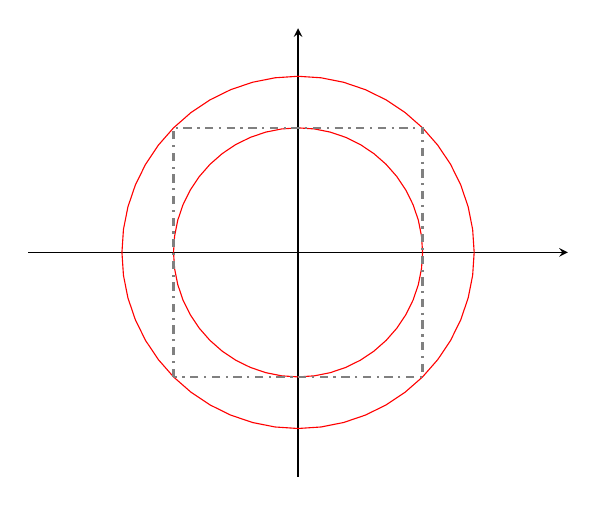
\begin{tikzpicture}
			\begin{axis}[axis lines=middle,xtick=\empty,ytick=\empty,axis equal,enlargelimits,xmax=1.5,ymax=1.5,xmin=-1.5,ymin=-1.5]
				%p=2
				\addplot[red,domain=-pi:0] ({(cos(deg(x)))},{(sin(deg(x))});
				\addplot[red,domain=0:pi] ({(cos(deg(x)))},{(sin(deg(x))});
				%p=2-larger
				\addplot[red,domain=-pi:0] ({(sqrt(2)*cos(deg(x)))},{((sqrt(2)*sin(deg(x))});
				\addplot[red,domain=0:pi] ({((sqrt(2)*cos(deg(x)))},{((sqrt(2)*sin(deg(x))});
				%p=inf
				\draw[thick,dashdotted,gray] (axis cs:-1,-1) rectangle (axis cs:1,1);
			\end{axis}
		\end{tikzpicture}
	\end{figure}
	since the circles in \(\left\lVert \cdot\right\rVert _\infty \) are squares.
\end{eg}

\begin{eg}
	For \(1\leq p, q\leq \infty \), we have \(L^p(\mathbb{R} , m)\)-\hyperref[def:norm]{norm} and \(L^q(\mathbb{R} , m)\)-\hyperref[def:norm]{norm} are not equivalent, even worse,
	we have that
	\[
		L^p(\mathbb{R} , m)\nsubseteq L^1(\mathbb{R} , m),\quad L^p(\mathbb{R} , m)\nsupseteq L^1(\mathbb{R} , m).
	\]
\end{eg}